\documentclass[tikz,border=3pt]{standalone}

\usepackage[T1]{fontenc}
\usepackage{libertine}
\usepackage{newtxmath}
\usepackage{fontawesome5}
\usepackage{xcolor}
\usetikzlibrary{arrows.meta,calc,positioning}

\renewcommand{\familydefault}{\sfdefault}

\definecolor{ink}{HTML}{20313F}
\definecolor{muted}{HTML}{667784}
\definecolor{line}{HTML}{8FA2AF}
\definecolor{blue}{HTML}{2A6F97}
\definecolor{bluefill}{HTML}{EAF3F8}
\definecolor{teal}{HTML}{2A9D8F}
\definecolor{tealfill}{HTML}{E8F6F3}
\definecolor{orange}{HTML}{D97745}
\definecolor{orangefill}{HTML}{FFF1E8}
\definecolor{slatefill}{HTML}{F4F7F9}

\tikzset{
  flow/.style={
    -{Latex[length=2.2mm,width=1.5mm]},
    draw=ink,
    line width=0.85pt,
    rounded corners=2pt
  },
  dataflow/.style={
    -{Latex[length=2.2mm,width=1.5mm]},
    draw=muted,
    line width=0.85pt,
    rounded corners=2pt
  },
  modelcard/.style={
    rounded corners=4pt,
    draw=blue,
    line width=0.9pt,
    fill=bluefill,
    minimum height=1.55cm,
    align=center,
    text=ink,
    inner xsep=6pt,
    inner ysep=5pt
  },
  scorecard/.style={
    rounded corners=4pt,
    draw=teal,
    line width=0.9pt,
    fill=tealfill,
    minimum height=1.55cm,
    align=center,
    text=ink,
    inner xsep=6pt,
    inner ysep=5pt
  },
  adaptcard/.style={
    rounded corners=4pt,
    draw=orange,
    line width=0.9pt,
    fill=orangefill,
    minimum height=1.55cm,
    align=center,
    text=ink,
    inner xsep=6pt,
    inner ysep=5pt
  },
  corpus/.style={
    rounded corners=4pt,
    draw=line,
    line width=0.85pt,
    fill=white,
    minimum height=1.38cm,
    align=center,
    text=ink,
    inner xsep=6pt,
    inner ysep=5pt
  },
  badge/.style={
    circle,
    minimum size=5.2mm,
    inner sep=0pt,
    text=white,
    font=\sffamily\bfseries\scriptsize
  },
  arrowlabel/.style={
    fill=white,
    text=muted,
    font=\sffamily\scriptsize,
    inner xsep=2.5pt,
    inner ysep=1pt,
    align=center
  }
}

\begin{document}
\begin{tikzpicture}[font=\sffamily, every node/.append style={outer sep=0pt}]
  % Phase backgrounds keep the two corpora's roles visually distinct.
  \filldraw[
    rounded corners=6pt,
    draw=blue!28,
    fill=bluefill!45,
    line width=0.65pt
  ] (-0.05,1.25) rectangle (10.65,4.75);
  \filldraw[
    rounded corners=6pt,
    draw=teal!28,
    fill=slatefill,
    line width=0.65pt
  ] (-0.05,-1.95) rectangle (18.25,1.45);

  \node[
    anchor=west,
    text=blue,
    fill=bluefill,
    rounded corners=2pt,
    inner xsep=4pt,
    inner ysep=1.5pt,
    font=\sffamily\bfseries\scriptsize
  ] at (0.22,4.47) {A \quad STYLE MODEL INDUCTION};
  \node[
    anchor=west,
    text=teal,
    fill=slatefill,
    rounded corners=2pt,
    inner xsep=4pt,
    inner ysep=1.5pt,
    font=\sffamily\bfseries\scriptsize
  ] at (3.35,1.18) {B \quad DATA SELECTION \& ADAPTATION};

  \node[corpus, text width=2.35cm] (small) at (1.48,2.62) {%
    {\color{blue}\large\faDatabase}\\[-1pt]
    {\scriptsize STYLE REFERENCE}\\[-1pt]
    \textbf{Small, high-quality\\dialogue corpus}
  };

  \node[modelcard, text width=2.82cm] (analysis) at (4.62,2.62) {%
    \textbf{Dialogue Feature\\Analysis}\\[2pt]
    {\scriptsize states \(\bullet\) strategies \(\bullet\) transitions}
  };

  \node[modelcard, text width=3.05cm] (modeling) at (8.68,2.62) {%
    \textbf{Bayesian Dialogue\\Modeling}\\[2pt]
    {\scriptsize transition \& observation probabilities}
  };

  \node[corpus, text width=2.70cm] (large) at (1.66,-0.62) {%
    {\color{muted}\large\faLayerGroup}\\[-1pt]
    {\scriptsize CANDIDATE POOL}\\[-1pt]
    \textbf{Large, general-purpose\\dialogue corpus}
  };

  \node[scorecard, text width=3.05cm] (scoring) at (6.05,-0.62) {%
    \textbf{Style Compatibility\\Scoring}\\[2pt]
    {\scriptsize \(\mathrm{Score}(r_t)\in[0,1]\)}
  };

  \node[adaptcard, text width=4.00cm] (adaptation) at (11.20,-0.62) {%
    \textbf{Preference Data Selection\\\& DPO Adaptation}\\[2pt]
    {\scriptsize \(\textit{chosen}\succ\textit{rejected}\)}
  };

  \node[
    rounded corners=4pt,
    draw=ink,
    line width=0.9pt,
    fill=ink,
    minimum height=1.50cm,
    text width=2.35cm,
    align=center,
    text=white,
    inner xsep=6pt,
    inner ysep=5pt
  ] (local) at (16.32,-0.62) {%
    {\large\faMicrochip}\\[-1pt]
    \textbf{Style-adapted\\local LLM}
  };

  % Number badges make the four modules easy to map to the method text.
  \node[badge, fill=blue] at ($(analysis.north west)+(0.18,-0.16)$) {1};
  \node[badge, fill=blue] at ($(modeling.north west)+(0.18,-0.16)$) {2};
  \node[badge, fill=teal] at ($(scoring.north west)+(0.18,-0.16)$) {3};
  \node[badge, fill=orange] at ($(adaptation.north west)+(0.18,-0.16)$) {4};

  % Style-reference path.
  \draw[flow] (small.east) -- (analysis.west);
  \draw[flow] (analysis.east) -- node[arrowlabel] {dialogue features} (modeling.west);

  % The learned Bayesian model and general-corpus candidates meet at scoring.
  \draw[flow, draw=blue]
    (modeling.south)
    -- (8.68,0.98)
    -- (6.05,0.98)
    -- node[arrowlabel, pos=0.67] {Bayesian dialogue model}
    (scoring.north);
  \draw[dataflow]
    (large.east)
    -- node[arrowlabel] {candidate responses}
    (scoring.west);

  % Scored candidates are converted to preferences and used for adaptation.
  \draw[flow, draw=teal]
    (scoring.east)
    -- node[arrowlabel] {scored candidates}
    (adaptation.west);
  \draw[flow, draw=orange]
    (adaptation.east)
    -- node[arrowlabel] {LoRA--DPO}
    (local.west);
\end{tikzpicture}
\end{document}
